% The tree of a DID's rotation keys, and the path a record carries.
\documentclass[border=12pt]{standalone}
% The look shared by the figures drawn with TikZ: the font and the colours
% of the Mermaid diagrams (mermaid.json). Built with xelatex, see AGENTS.md.
\usepackage[no-math]{fontspec}
\setmainfont{Lato}
\setsansfont{Lato}
\renewcommand{\familydefault}{\sfdefault}
\usepackage{amsmath}
\usepackage{tikz}
\usetikzlibrary{arrows.meta,positioning,calc,fit,backgrounds}

\definecolor{navy}{HTML}{1F3A5F}
\definecolor{ink}{HTML}{1F2A37}
\definecolor{muted}{HTML}{5C6B7E}
\definecolor{blueFill}{HTML}{EEF4FB}
\definecolor{blueLine}{HTML}{5B7FAE}
\definecolor{greenFill}{HTML}{E3F4E8}
\definecolor{greenLine}{HTML}{2F8F4E}
\definecolor{amberFill}{HTML}{FDF1DC}
\definecolor{amberLine}{HTML}{C98A1B}
\definecolor{violetFill}{HTML}{F3EFFC}
\definecolor{violetLine}{HTML}{7B61B8}
\definecolor{greyFill}{HTML}{F6F8FB}
\definecolor{greyLine}{HTML}{C3CCD7}

\tikzset{
  every picture/.style={font=\small, color=ink, line cap=round},
  base/.style={rounded corners=3pt, line width=0.7pt, align=center, inner sep=5pt},
  plain/.style={base, draw=greyLine, fill=white},
  public/.style={base, draw=blueLine, fill=blueFill},
  secret/.style={base, draw=violetLine, fill=violetFill},
  result/.style={base, draw=greenLine, fill=greenFill},
  carried/.style={base, draw=amberLine, fill=amberFill},
  strong/.style={base, draw=navy, fill=navy, text=white, font=\small\bfseries},
  op/.style={base, draw=navy, fill=white, line width=0.9pt, font=\small\bfseries},
  flow/.style={-{Stealth[length=2.2mm]}, draw=muted, line width=0.7pt},
  link/.style={draw=muted, line width=0.7pt},
  data/.style={font=\footnotesize, fill=white, inner sep=1.5pt, text=ink},
}

\begin{document}
\newcommand{\swatch}[1]{\tikz[baseline=0pt]\draw[#1, rounded corners=1.5pt] (0,-0.02) rectangle (0.5,0.27);}
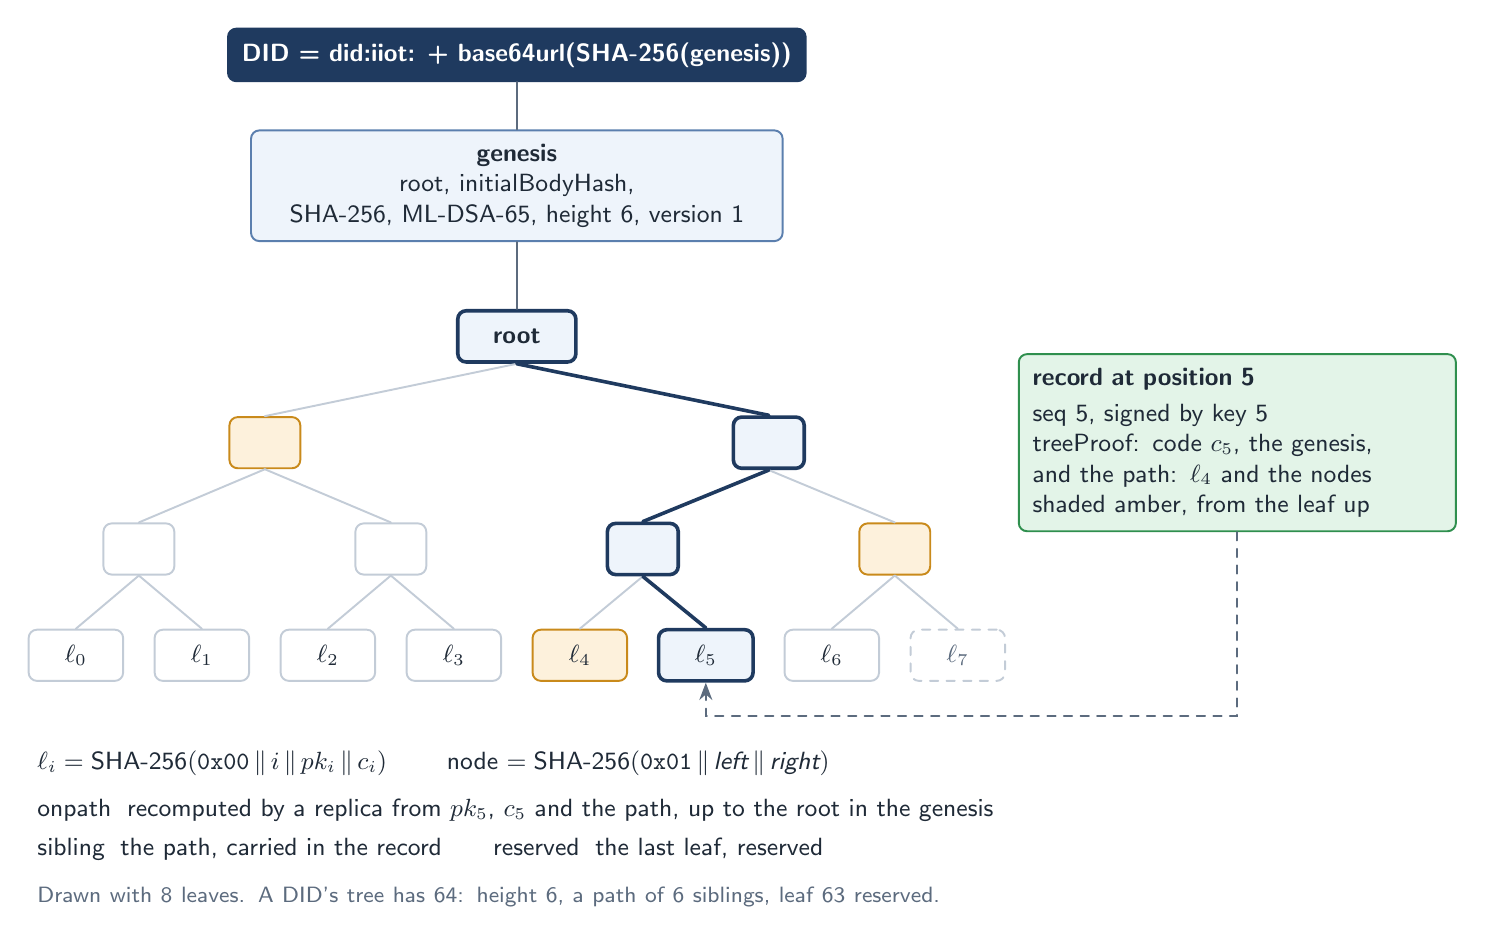
\begin{tikzpicture}[
  node/.style={plain, minimum width=9mm, minimum height=6.5mm, inner sep=2pt},
  onpath/.style={public, draw=navy, line width=1.3pt, minimum width=9mm, minimum height=6.5mm, inner sep=2pt},
  sibling/.style={carried, minimum width=9mm, minimum height=6.5mm, inner sep=2pt},
  reserved/.style={node, draw=greyLine, dashed, text=muted},
  leafw/.style={minimum width=12mm},
  edge/.style={link, draw=greyLine},
  pathedge/.style={draw=navy, line width=1.3pt},
]
  % 8 leaves drawn; the tree has 64
  \foreach \i in {0,...,7} \coordinate (L\i) at (\i*1.6,0);
  \node[node, leafw] (l0) at (L0) {$\ell_0$};
  \node[node, leafw] (l1) at (L1) {$\ell_1$};
  \node[node, leafw] (l2) at (L2) {$\ell_2$};
  \node[node, leafw] (l3) at (L3) {$\ell_3$};
  \node[sibling, leafw] (l4) at (L4) {$\ell_4$};
  \node[onpath, leafw] (l5) at (L5) {$\ell_5$};
  \node[node, leafw] (l6) at (L6) {$\ell_6$};
  \node[reserved, leafw] (l7) at (L7) {$\ell_7$};

  \node[node] (a0) at ($(l0)!0.5!(l1)+(0,1.35)$) {};
  \node[node] (a1) at ($(l2)!0.5!(l3)+(0,1.35)$) {};
  \node[onpath] (a2) at ($(l4)!0.5!(l5)+(0,1.35)$) {};
  \node[sibling] (a3) at ($(l6)!0.5!(l7)+(0,1.35)$) {};
  \node[sibling] (b0) at ($(a0)!0.5!(a1)+(0,1.35)$) {};
  \node[onpath] (b1) at ($(a2)!0.5!(a3)+(0,1.35)$) {};
  \node[onpath, minimum width=15mm, font=\small\bfseries] (root) at ($(b0)!0.5!(b1)+(0,1.35)$) {root};

  \foreach \p/\c in {a0/l0, a0/l1, a1/l2, a1/l3, a2/l4, a3/l6, a3/l7, b0/a0, b0/a1, b1/a3, root/b0}
    \draw[edge] (\p.south) -- (\c.north);
  \foreach \p/\c in {a2/l5, b1/a2, root/b1}
    \draw[pathedge] (\p.south) -- (\c.north);

  \node[public, above=0.85cm of root, text width=6.4cm] (gen)
    {\textbf{genesis}\\ root, initialBodyHash,\\ SHA-256, ML-DSA-65, height 6, version 1};
  \node[strong, above=0.6cm of gen] (did)
    {DID = did:iiot: + base64url(SHA-256(genesis))};
  \draw[link] (root.north) -- (gen.south);
  \draw[link] (gen.north) -- (did.south);

  % the record at position 5
  \node[result, right=1.1cm of a3, anchor=west, text width=5.2cm, align=left] (rec) at (a3.east |- b1) {%
    \textbf{record at position 5}\\[2pt]
    seq 5, signed by key 5\\
    treeProof: code $c_5$, the genesis,\\
    and the path: $\ell_4$ and the nodes\\
    shaded amber, from the leaf up};
  \draw[flow, dashed] (rec.south) |- ($(l5.south)+(0,-0.42)$) -- (l5.south);

  % formulas and legend
  \node[anchor=north west, align=left, text width=13cm] at ($(l0.south west)+(0,-0.75)$) {%
    $\ell_i = \text{SHA-256}(\texttt{0x00} \,\Vert\, i \,\Vert\, pk_i \,\Vert\, c_i)$
    \qquad node $= \text{SHA-256}(\texttt{0x01} \,\Vert\, \textit{left} \,\Vert\, \textit{right})$\\[6pt]
    \swatch{onpath}\;
    recomputed by a replica from $pk_5$, $c_5$ and the path, up to the root in the genesis\\[3pt]
    \swatch{sibling}\;
    the path, carried in the record\qquad
    \swatch{reserved}\;
    the last leaf, reserved\\[6pt]
    {\footnotesize\color{muted} Drawn with 8 leaves. A DID's tree has 64: height 6, a path of 6 siblings, leaf 63 reserved.}};
\end{tikzpicture}
\end{document}
